% !TEX encoding = UTF-8 Unicode

\documentclass{standalone}

% packages
\usepackage{float}
\usepackage{tabu}
\usepackage{booktabs}
\usepackage{graphicx}
\usepackage{caption}
\usepackage[export]{adjustbox}
\usepackage[utf8]{inputenc}
%\usepackage[active,pdftex,tightpage]{preview}
\usepackage{newtxtext,newtxmath}
\usepackage[percent]{overpic}

\begin{document}

%\sf
\scriptsize
\centering 

%Shallow overland water depth $(m)$ simulated by SIMWE for a $10 min$ event with $50~mm~hr^{-1}$}

\begin{tabular}{m{0.5\textwidth} m{0.5\textwidth}}

% simwe depth
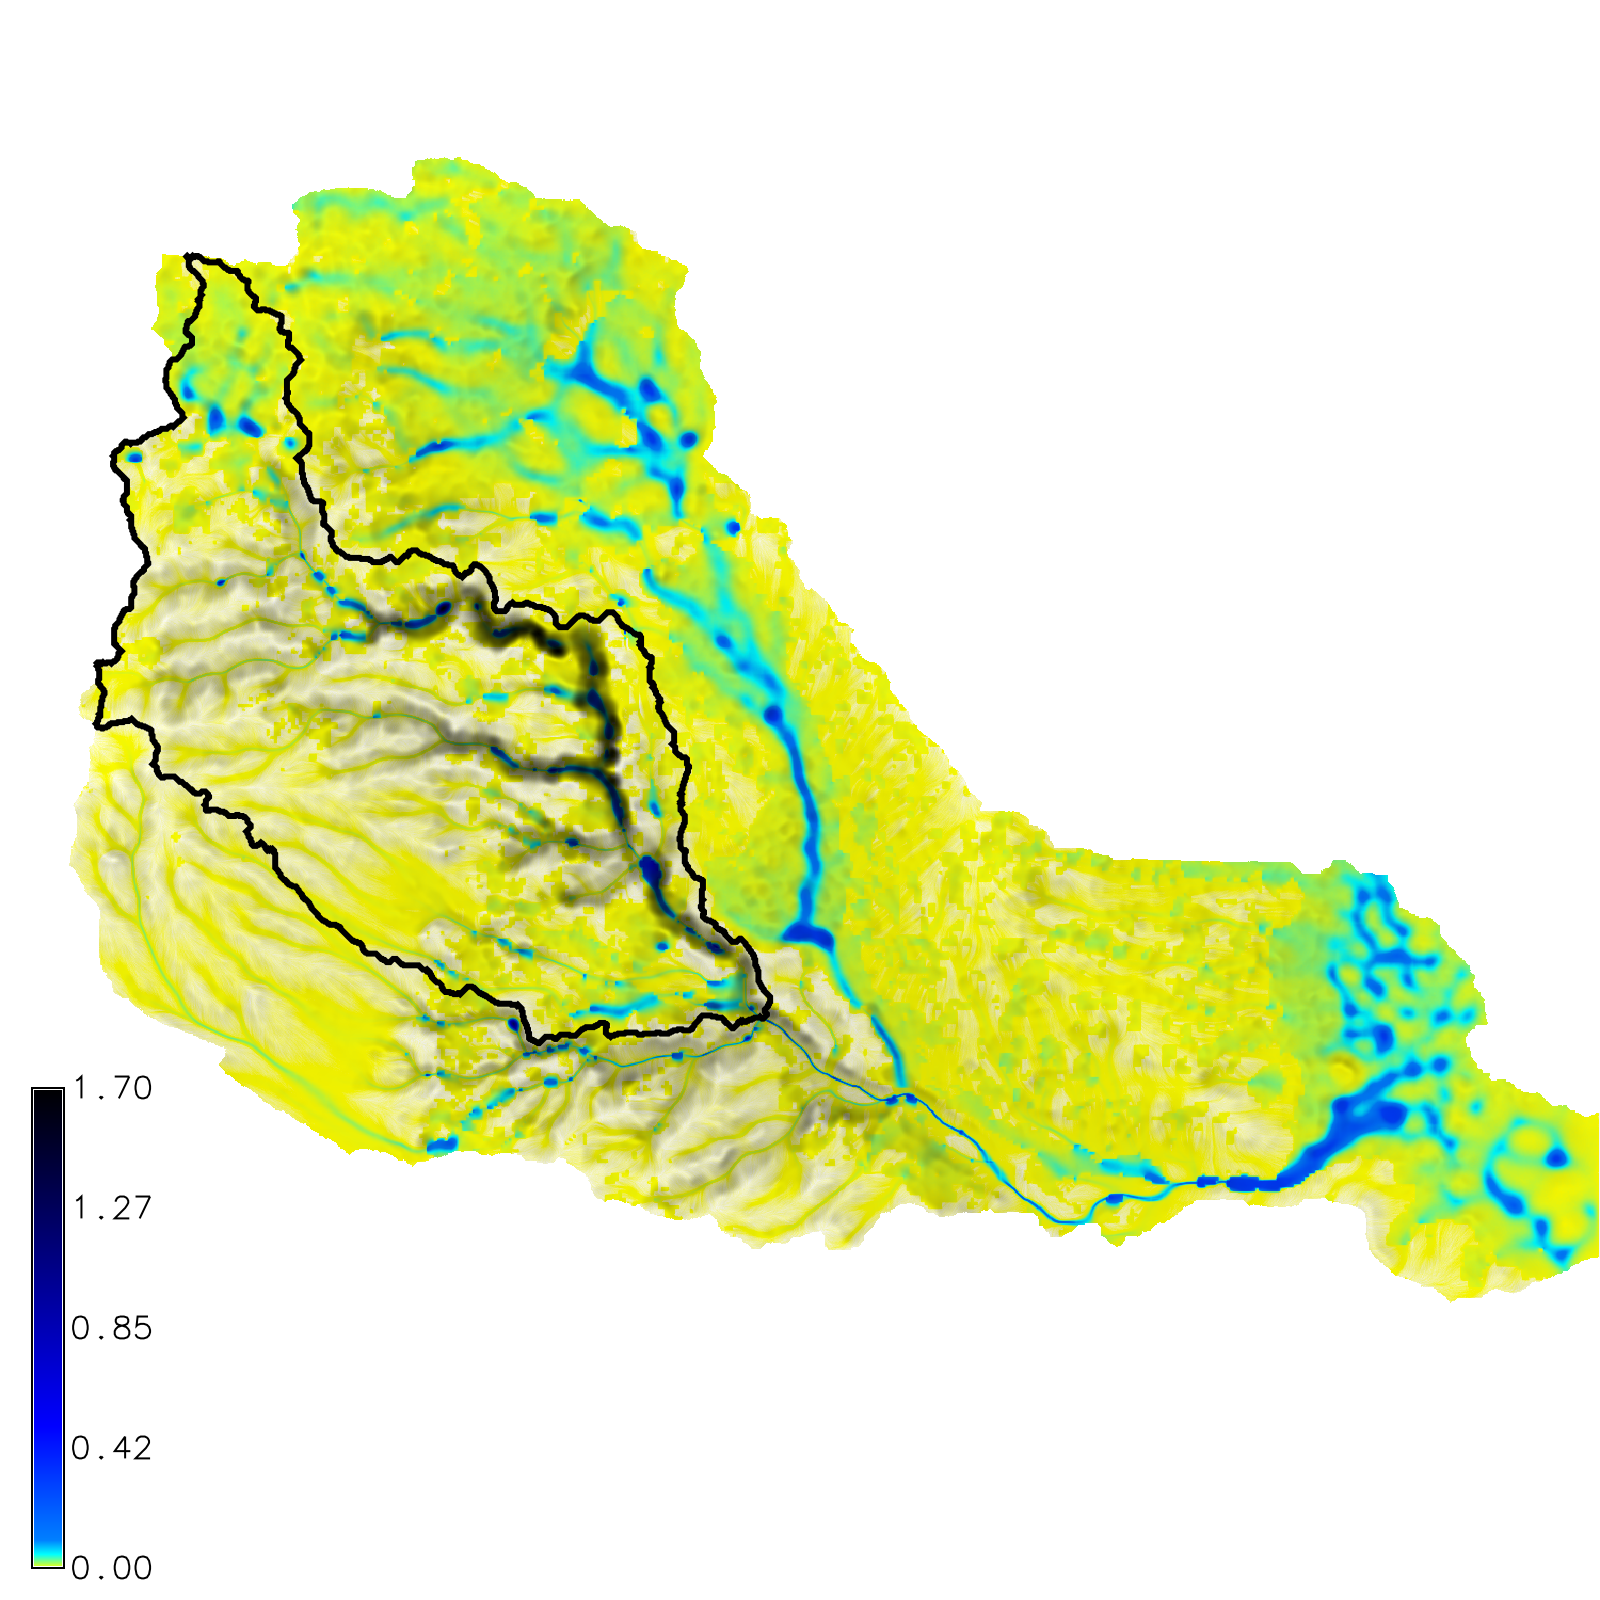
\includegraphics[height=50mm]{../../images/sample_data/depth_subwatersheds.png}&
% rusle flowacc
\begin{overpic}[height=50mm]{../../images/sample_data/flowacc_subwatersheds.png}
\put(-26,0){
\includegraphics[height=100mm,center]{../../images/sample_data/map_elements.png}}  
\end{overpic}\\
\multicolumn{1}{c}{a.}&
\multicolumn{1}{c}{b.}\\
\\
\\
% simwe erdep
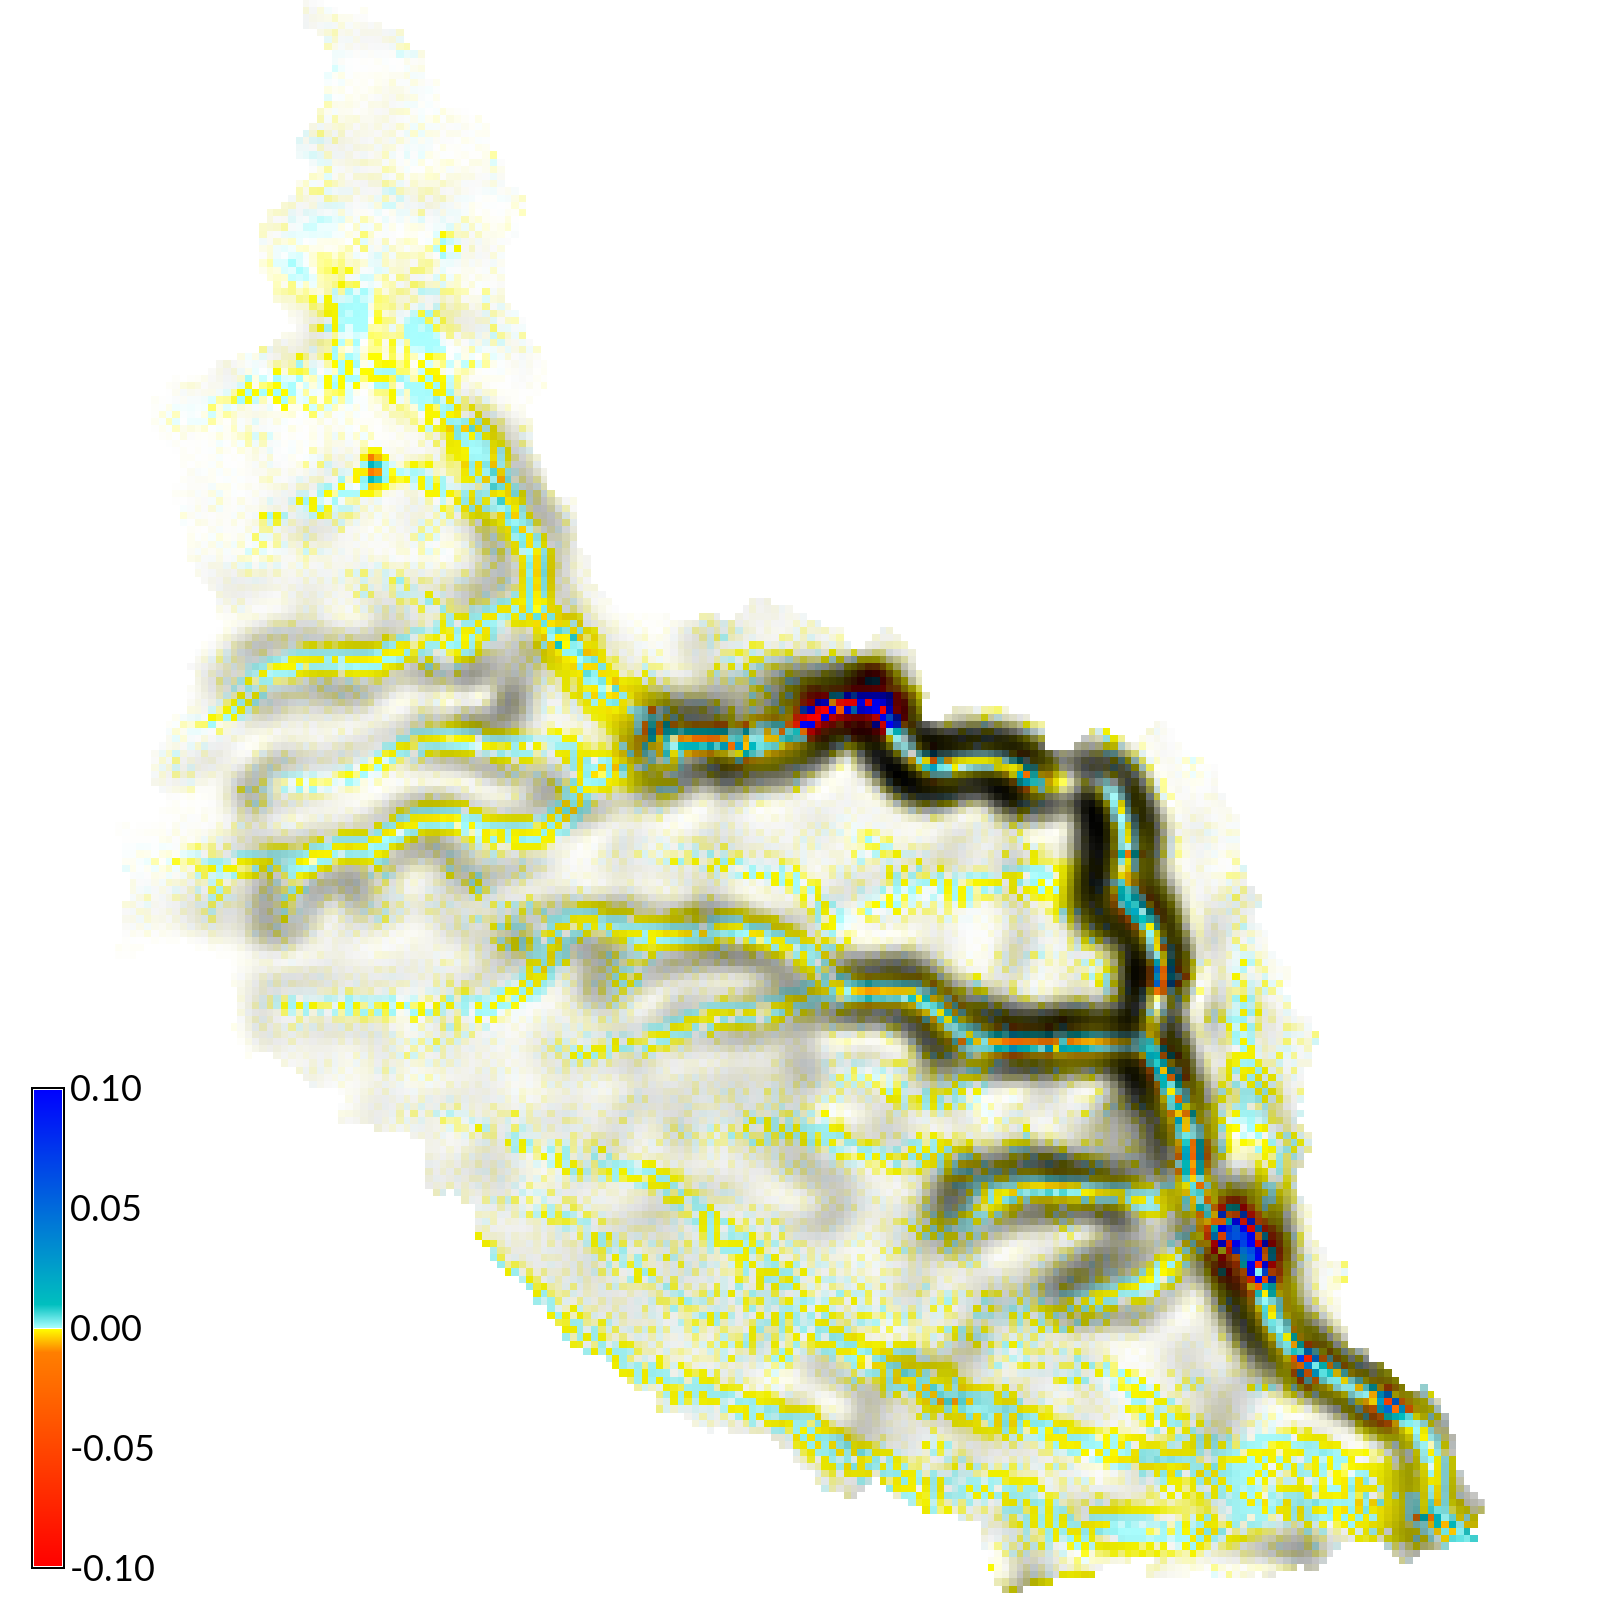
\includegraphics[height=50mm,center]{../../images/sample_data_detail/erosion_deposition_2012.png}&
% rusle sedflow
\begin{overpic}[height=50mm,center]{../../images/sample_data_detail/sediment_flow_2012.png}
\put(-22,-12){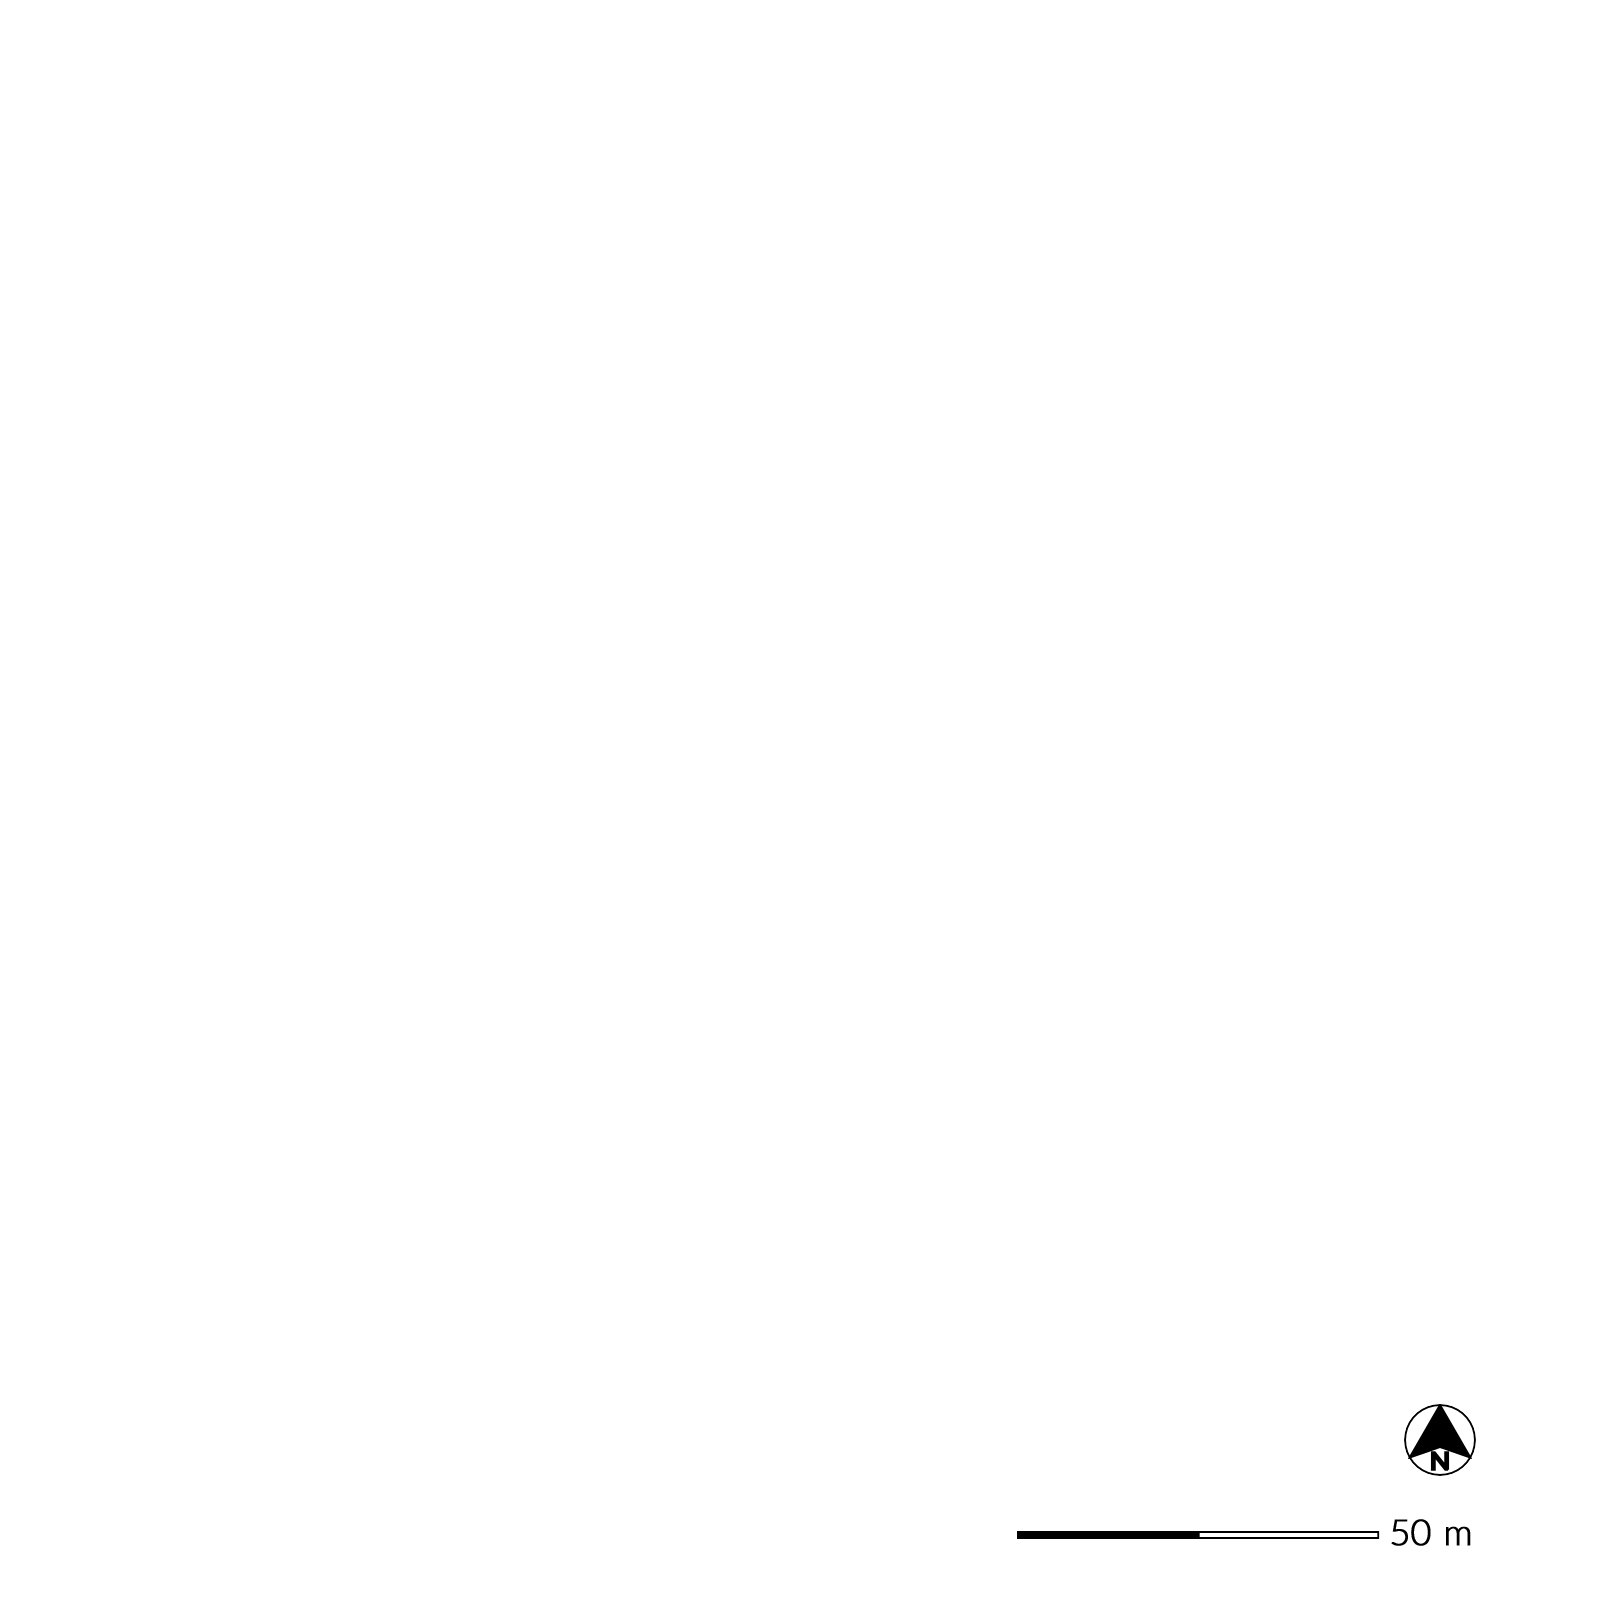
\includegraphics[height=100mm,center]{../../images/sample_data/map_elements_detail.png}}  
\end{overpic}\\
\\
\\
\multicolumn{1}{c}{c.}&
\multicolumn{1}{c}{d.}\\
%
\end{tabular}

\end{document}
